% QTML 2026 POSTER abstract (non-archival, non-anonymous). One page (poster limit).
% Condensed from abstract_qtml.tex. Format: PDF, single column, single-spaced, 11pt.
\documentclass[11pt]{article}
\usepackage[letterpaper,margin=1in]{geometry}
\usepackage[T1]{fontenc}
\usepackage{amsmath,amssymb}
\usepackage{graphicx}
\usepackage[hidelinks]{hyperref}
\graphicspath{{../figures/}}
\pagestyle{empty}
\setlength{\parskip}{3pt}

\begin{document}
\begin{center}
{\large\bfseries \textsc{SimCert}: A Classical-Simulability Audit of Trained Quantum-NLP Text Classifiers}\\[5pt]
{\normalsize Tanvir Ahmed$^{1}$}\\[2pt]
{\small $^{1}$North South University, Dhaka, Bangladesh \quad\textbullet\quad tanvir.ahmed32@northsouth.edu}\\[2pt]
{\small Submission type: poster \quad\textbullet\quad Track: Quantum NLP; Benchmarking and Complexity}
\end{center}
\vspace{1pt}

Quantum natural language processing (QNLP) models, from compositional DisCoCat circuits to quantum
self-attention networks and all-quantum token mixers, are promoted for a quantum benefit on text
classification. That benefit is usually argued from accuracy, yet whether a \emph{trained} QNLP
circuit ever leaves the efficiently classically-simulable regime is rarely tested. We ask which
published QNLP results survive a classical surrogate of the trained circuit.

We introduce \textsc{SimCert}, an open and model-agnostic protocol. It re-simulates each trained
circuit as a bond-dimension-$\chi$ matrix product state, sweeps $\chi$, and records the smallest
value $\chi^\star$ at which a classical surrogate recovers the model's own predictions, together with
an entanglement-removal ablation, the state entanglement entropy, a geometric-difference kernel test,
and a data-reuploading spectral test. A single audit consumer treats every model uniformly through a
common circuit representation, including a mixed-state purification path for models whose readout is a
reduced density matrix.

We audit five published architectures, namely DisCoCat as realised in lambeq, the quantum
self-attention models QSANN and QMSAN, the all-quantum token mixer CLAQS, and a variational reference
classifier, across four datasets and up to ten qubits. A classical surrogate recovers the predictions
at small and non-growing bond dimension: attention and mixer models at $\chi{=}1$, a product state,
and the compositional model at $\chi{=}2$. As we grow the qubit count on a fixed task, $\chi^\star$
stays flat while the exact-MPS bound $2^{n/2}$ grows exponentially (figure). The circuits carry
entanglement, with mean bipartite entropy from about $0.1$ to $1.3$ nats, but removing it barely moves
the result, so the entanglement is present without being load-bearing for the decision. The one
exception is the compositional model, whose grammar cups make $\chi{=}1$ collapse toward chance.

We read this cautiously: it suggests the quantum resource is not the operative ingredient at the
scales these models are tested, not that QNLP is classically simulable in general. We release the
harness and phrase the finding as a protocol and a set of questions for QNLP model and benchmark
design, chief among them which architectural choices, if any, make $\chi^\star$ grow with system size.

\vspace{2pt}
\begin{center}
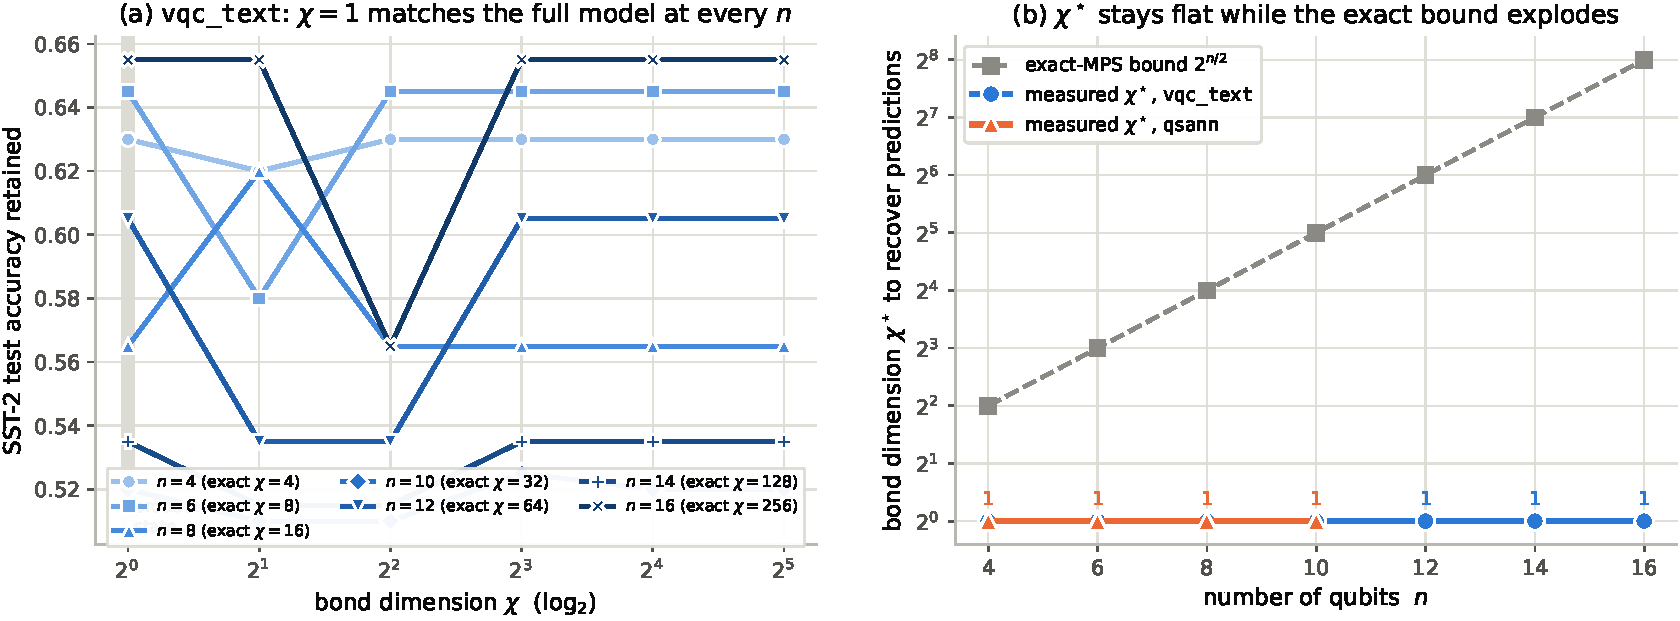
\includegraphics[width=0.72\linewidth]{scaling.pdf}\\
{\small $\chi^\star$ stays flat at $1$ as the reference model grows from four to ten qubits (right),
while the exact-MPS bound $2^{n/2}$ grows exponentially (grey). Left: accuracy is flat in $\chi$ at
every size.}
\end{center}

\end{document}
